\documentclass[12p]{article}
\usepackage[utf8]{inputenc}
\usepackage{amssymb}
\usepackage{graphicx}
\usepackage{graphicx}
\usepackage{amsmath}
\usepackage[inkscapeformat=png]{svg}
\usepackage{wasysym}
\graphicspath{ {./images/} }
\usepackage{subcaption}
\usepackage{listings}
\usepackage{csquotes}
\usepackage{wrapfig}
\usepackage[colorlinks, bookmarks=false, linkcolor=black, urlcolor=blue, citecolor=black]{hyperref}
\usepackage{matlab-prettifier}
\usepackage[top=2.5cm, bottom=3 cm, left=3.5cm, right=3.5cm]{geometry}
\usepackage{xcolor}

% \pagecolor{black}
% \color{white}

\newcommand*{\proj}{\text{Proj}}
\newcommand*{\es}{\mathcal{E}}

\title{MATH-329 Nonlinear optimization
Homework 3: Constrained optimization}
\author{Alix Pelletier 346750 \\ Vlad Burca 344876 \\ Ismail Bouhaj 326480}
\date{11/2023}
\begin{document}
\maketitle 
\section*{Part 1 : Projections to cones and stopping criteria in constrained optimization.}
\subsection*{Question 1} \hfil\par
Since \(Q\) is non-empty, Let \(x_0\in Q\). Then by definition of the minimizer, we have:
\[
  \min_{x\in Q} \frac{1}{2}\|x-z\|^2 \leq \frac{1}{2}\|x_0-z\|^2
\]

Inspired by this, let us define the space \(Q'\subseteq Q\) as the intersection of \(Q\) with the closed ball \(\bar B(\|x_0-z\|,z)\) of center \(z\) and radius \(\|x_0-z\|\):
\[
    Q'=Q\cap \bar B(\|x_0-z\|,z)  
\]

We have \(Q'\neq \emptyset\) since \(x_0\in Q'\). Moreover, \(Q'\) is closed since it is the intersection of two closed sets. Finally, \(Q'\) is bounded since it is contained in the closed ball \(\bar B(\|x_0-z\|,z)\). Therefore, \(Q'\) is compact. By Weierstrass, the function \(f(x)=\frac{1}{2}\|x-z\|^2\) attains its minimum on \(Q'\). So the set:
\[
    \proj_{Q'}(z)=\left\{x\in Q': \frac{1}{2}\|x-z\|^2=\min_{y\in Q'}\frac{1}{2}\|y-z\|^2\right\}    
\]
is well-defined and non-empty.

We want to show that \(\proj_{Q'}(z)=\proj_Q(z) \). Let \(x\in Q\setminus Q'\). Then:
\[
    \|x-z\|>\|x_0-z\|\implies 
\]
\[
    \frac{1}{2}\|x-z\|^2>\frac{1}{2}\|x_0-z\|^2\geq \min_{y\in Q'}\frac{1}{2}\|y-z\|^2
\]
 
So the minimizer of \(\frac{1}{2}\|y-z\|^2 \) on \(Q'\) is also the minimizer of \(\frac{1}{2}\|y-z\|^2\) on \(Q\). Therefore, \(\proj_{Q'}(z)=\proj_Q(z) \).

\subsection*{Question 2} 
Let \(\es:=\mathbb{R};\ S:=\{-1,1\};\ z:=0\). Then clearly \(S\) is closed (union of 2 singletons). Moreover, we have:
\begin{align*}
    \frac{1}{2}\|z-s\|^2&=\frac{1}{2}\|s\|^2=\frac{1}{2}\ \text{for all}\ s\in S \implies \\
\end{align*}
\[
    \proj_S(z)=\{1,-1\} 
\]

\subsection*{Question 3} 

\subsubsection*{\textbf{\( \text{Proj}_C(z) = \{0\} \implies z \in C^\circ \):}}\hfil\par 
Assume \( \text{Proj}_C(z) = \{0\} \). This implies the point in \( C \) closest to \( z \) is the origin. So for any \( x \in C \):
 \begin{align*}
        \frac{1}{2} \|x - z\|^2 &\geq \frac{1}{2} \|0 - z\|^2 \\
        \|x\|^2-2\langle x, z\rangle +\|z\|^2 &\geq \|z\|^2 \\
        \|x\|^2  -2\langle x, z\rangle &\geq 0\\
 \end{align*}

 Now if \(\langle x, z\rangle > 0\), for some \(x\) then we have:
 \[
   \lambda:=\frac{\langle x, z\rangle}{\|z\|^2}>0\implies \lambda x\in C 
 \]

 But then, plugging \(\lambda x\) in the inequality above, we get:
\[
    \lambda^2\|x\|^2-2\lambda\langle x, z\rangle \geq 0\iff      
\]
\[
    \left(\frac{\langle x, z\rangle}{\|z\|^2}\right)^2\|x\|^2-2\frac{\langle x, z\rangle}{\|z\|^2}\langle x, z\rangle \geq 0\iff
\]
\[
  -\frac{\langle x, z\rangle^2 }{\|x\|^2} \geq 0 
\]

Which is clearly a contradiction. Therefore, we must have \(\langle x, z\rangle \leq 0\) for all \(x\in C\). This implies \(z\in C^\circ\), by definition.
\subsubsection*{\( z \in C^\circ  \implies \text{Proj}_C(z) = \{0\} \):}\hfil\par
Assume \( z \in C^\circ \). We want to show that for all \(x\in C\setminus\{0\}\) we have: 
\[
    \frac{1}{2} \|x - z\|^2 > \frac{1}{2} \|0 - z\|^2 
\]

By the above calculations this is equivalent to showing that for all \(x\in C\setminus\{0\}\) we have:
\[
    \|x\|^2  -2\langle x, z\rangle > 0  
\]

But this is true since \(z\in C^\circ\), so \(\langle x, z\rangle\leq 0\) for all \(x\in C\) and \(x\neq 0\). Therefore, we have:
\[
  \proj_C(z)=\{0\}  
\]
\subsection*{Question 4} \hfil\par
We know from class that \(x^*\in S\) is a stationary point of \(f\) if and only if \(-\nabla f(x^*)\in (T_{x^*}S)^\circ\). By Question 3, this is equivalent to:
 \[\text{Proj}_{T_{x^*}S}(-\nabla f(x^*))=\{0\}\]
\pagebreak
\subsection*{Question 5}\hfil\par 
\subsubsection*{(a)\quad \(v\in \proj_C(z)\implies \langle v, z-v\rangle = 0\):}\hfil\par
Let:

\begin{align*}
    g: \es &\to \quad \quad \mathbb{R}\\
    x &\mapsto \frac{1}{2}\|x-z\|^2
\end{align*} 
    
Then \(g\) is differentiable and for\(h\in \mathbb{R}\) and \(v\in\es\) we have:
\begin{align*}
g(x+hv)=\frac{1}{2}\|x+hv-z\|^2&=\frac{1}{2}\|x-z\|^2+h\langle v, x-z\rangle+\frac{h^2}{2}\|v\|^2\\
&=g(x)+h\langle v, x-z\rangle+O(h^2)\implies         
\end{align*}
\[
  \nabla g(x)= x-z 
\]
If \(v\in \proj_C(z)\) then \(v\) is a stationary point of \(g\) (as \(v\) is a global minimum of \(g\)). Therefore, we have: 
\[
  \langle \nabla g(v), w\rangle \geq 0, \quad  \forall\ w\in T_vC
\]
\[
  \langle v-z, w\rangle \geq 0, \quad  \forall\ w\in T_vC   
\]
It is clear that if we show that \(v,\ -v \in T_vC\) we are done. But this is true since \(v\in C\) and \(C\) is a cone.

Let \(\left((1-\frac{1}{n})v\right)_{n\in \mathbb{N}^*}\subseteq C\), \(\left((1+\frac{1}{n})v\right)_{n\in \mathbb{N}^*}\subseteq C\) then: 
\[
  \lim_{n\to \infty}\left((1-\frac{1}{n})v\right)=v,\quad \lim_{n\to \infty}\left((1+\frac{1}{n})v\right)=v 
\]
and:
\[
  \lim_{n\to \infty}\left(\frac{(1-\frac{1}{n})v-v}{\frac{1}{n}}\right)=\lim_{n\to \infty}\left(\frac{-\frac{1}{n}v}{\frac{1}{n}}\right)=-v 
\]
\[
    \lim_{n\to \infty}\left(\frac{(1+\frac{1}{n})v-v}{\frac{1}{n}}\right)=\lim_{n\to \infty}\left(\frac{\frac{1}{n}v}{\frac{1}{n}}\right)=v 
\]
Therefore, by the definition of the tangent cone \(v,\ -v \in T_vC\). So we have:
\begin{align*}
    \langle v-z, v\rangle &\geq 0\\
    \langle v-z, -v\rangle &\geq 0 \implies \\
    -\langle v-z, v\rangle &\geq 0
\end{align*}

So we have:
\[
    \langle v, z-v\rangle = 0  
\]
\subsubsection*{(b)\quad \(v_1,\ v_2\in \proj_C(z)\implies \|v_1\|=\|v_2\|\):}\hfil\par
By part (a), we have:
\[
    \langle v_1, z-v_1\rangle = 0 \implies \|v_1\|^2=\langle v_1, v_1\rangle=\langle v_1, z\rangle
\]
\[
    \langle v_2, z-v_2\rangle = 0 \implies \|v_2\|^2=\langle v_2, v_2\rangle=\langle v_2, z\rangle
\]
Since both are minimizers of \(\frac{1}{2}\|x-z\|^2\), we have:
\[
    \frac{1}{2}\|v_1-z\|^2= \frac{1}{2}\|v_2-z\|^2  \implies
\]
\[
  \|v_1\|^2-2\langle v_1, z\rangle+\|z\|^2=\|v_2\|^2-2\langle v_2, z\rangle+\|z\|^2\implies  
\]
\[
  \|v_1\|^2=\|v_2\|^2\implies \|v_1\|=\|v_2\|
\]
\subsection*{Question 6} 

We present an example where the function \( q(x) = \lVert \text{Proj}_{T_xS}(-\nabla f(x)) \rVert \) is discontinuous on the set \( S \). Consider the following:

\textbf{Function \( f \) and Set \( S \):}
\begin{itemize}
    \item Function \( f \): Define \( f: \mathbb{R} \rightarrow \mathbb{R} \) as \( f(x) = -x^2 \). Its gradient is \( \nabla f(x)=f'(x) = -2x \).
    \item Set \( S \): Define \( S := [0,1]\subseteq\mathbb{R}\).
\end{itemize}
First, let's compute \(T_xS\) for all \(x\in S\). We have: 
\begin{itemize}
    \item \(x\in(1,0)\). Then \(x\) is in the interior of \(S\) and \(T_xS=\mathbb{R}\), by example 7.10. from the lecture notes. 
    \item \(x=0\). Then 0 is on the boundary of \(S\) and \(T_0S=[0,+\infty)\), by example 7.11. from the lecture notes (we can see 0 as the boundary for the half-space \(x\geq 0\) and locally around 0 the two spaces are the same. We conclude by the fact that the tangent cone is a local property, as any sequence \(x_k\to 0^+\) will be contained in \((0,1)\), for \(k\) big enough). 
    \item \(x=1\). Then 1 is on the boundary of \(S\) and \(T_1S=(-\infty,0]\) (same reasoning as above, but with the half space \(x\leq 1\)).

\end{itemize}
Now, let's compute \(\text{Proj}_{T_xS}(-\nabla f(x))\) for all \(x\in S\). We have:
\begin{itemize}
    \item \(x\in(0,1)\). Then \(\text{Proj}_{T_xS}(-\nabla f(x))=\{-\nabla f(x)\}\), since \(T_xS=\mathbb{R}\). So:
    \[
        q(x)=\|2x\|=2x
    \]
    \item \(x=0\). Then \(\text{Proj}_{T_0S}(-\nabla f(0))=\{0\}\), since \(T_0S=[0,+\infty)\) and \(-f'(0)=0\). So:
    \[
        q(0)=\|0\|=0    
    \]
    \item \(x=1\). Then \(\text{Proj}_{T_1S}(-\nabla f(1))=\{0\}\), since \(T_1S=(-\infty,0]\) and \(-f'(1)=2\). So:
    \[
        q(1)=\|0\|=0    
    \]

\end{itemize}

So:
\[
        q(x)=\begin{cases}
            2x & \text{if } x\in[0,1)\\
            0 & \text{if }  x=1
        \end{cases}    
\]

Clearly, \(q\) is not continuous at \(x=1\).
\subsection*{Question 7} \hfil\par

By example 7.14. from the lecture notes, we have:
\[
    T_xS=\left\{v\in \mathbb{R}: \langle v,x \rangle =0\right\}, \quad \forall\ x\in S
\]

For all \(x=(x_1, x_2)\in S\), let \(x^\perp=(x_2, -x_1)\in S\), then it is clear that:
\[
    \langle x, x^\perp\rangle =0\implies x^\perp\in T_xS
\]

Moreover, by a simple argument over the dimensionality of \(T_xS\) and \(\text{span}(x^\perp)\), we have:
\[
    T_xS= \text{span}(x^\perp)
\]

Since \(T_xS\) is a sub-vector space of \(\mathbb{R}^2\), of dimension 1 (\(\{x^\perp\}\) is an orthogonal basis), we have:
\[
    \text{Proj}_{T_xS}(-\nabla f(x))=\text{Proj}_{\text{span}(x^\perp)}(-\nabla f(x))=\left\{\frac{\langle -\nabla f(x), x^\perp\rangle}{\|x^\perp\|^2}x^\perp\right\}=\left\{-\langle \nabla f(x), x^\perp\rangle x^\perp\right\}
\]

So:
\[
  q(x)=\|- \langle \nabla f(x), x^\perp\rangle x^\perp\|=\|- \langle \nabla f(x), (x_2, -x_1)\rangle (x_2, -x_1)\|=|\langle \nabla f(x), (x_2, -x_1)\rangle|
\]

Which is clearly a continuous map as it is a composition of continuous maps (\(\nabla f\) is continuous by assumption).

\subsection*{Question 8} \hfil\par

Consider \( \es = \mathbb{R}^n \) with a continuously differentiable function \( h: \mathbb{R}^n \rightarrow \mathbb{R}^p \) and \( S = \{x \in \mathbb{R}^n : h(x) = 0\} \), assuming LICQ holds for all \( x \) in \( S \).

\subsubsection*{(a) \(T_xS\)?}\hfil\par
From the lecture notes, we have that if LICQ holds for \(x\in S\) then:
\[
  T_xS=F_xS=\left\{v\in \es \ : \ \langle\nabla h_i(x),v\rangle=0;\ \forall i\in\{1,2,\dots,p\}\right\}  
\]
\subsubsection*{(b)}\hfil\par
Let \(H(x)\in\mathbb{R}^{p\times n}\) such that:
\[
  H(x)=\begin{pmatrix}
    \nabla h_1(x)^T\\
    \nabla h_2(x)^T\\
    \vdots\\
    \nabla h_p(x)^T  
    \end{pmatrix}
\]

Then we can rewrite \(T_xS\) as:
\[
  T_xS=\left\{v\in \es \ : \ H(x)v=0\right\} =\ker H(x)  
\]

As \(T_xS\) is a sub-vector space of \(\es\) of dimension \(n-p\) (since all the lines of \(H(x)\) are linearly independent), we know that the projection of \(z\in \es\) exists and is unique. 

By SVD, there exist \(V\in\mathbb{R}^{n\times n}\) and \(U\in\mathbb{R}^{p\times p}\) orthogonal matrices and \(D\in\mathbb{R}^{p\times n}\) such that:
\[
  UH(x)V=D
\]
\[
  D=\begin{pmatrix}
    \begin{matrix}
    \sigma_1 &  &  & \\
     & \sigma_2 &  & \\
     &  & \ddots & \\
     &  &  & \sigma_p\\
    \end{matrix} & O_{p\times(n-p)}\\
    \end{pmatrix}  
\]

Where \(\sigma_1,\sigma_2,\dots,\sigma_p\) are the singular values of \(H(x)\).

Let \(V=(v_1, v_2, \dots v_n)\), where \(v_i\in \es\). Then we can see that \(\{v_{n-p+1},v_{n-p+2},\dots,v_{n}\}\) form an orthonormal basis of \(\ker H(x)\). So we have, based on the definition of the projection, for a sub-vector space:
\[
  \proj_{\ker H(x)}(z)=\left\{\sum_{i=n-p+1}^{n}\langle z, v_i\rangle v_i\right\}
\]
\subsubsection*{(c)}\hfil\par
We can easily see that \(q\) is a continuous function, as it is a composition of continuous functions. Since \(H(x)\) is continuous, we expect that the (normalized) basis elements obtained through Gram-Schmidt (so through SVD) to not change too much. And since \(H(x)\) is always of full rank \(p\), we expect that \(\| \proj_{\ker H(x)}(z)\|\) to be continuous. Then \(q\) is just this composed with \(\nabla f\) which is continuous by assumption. So \(q\) is continuous.
\newpage


\section*{Part 2 : A Frank-Wolfe algorithm} 


\subsection*{Question 1}\hfil\par
we can see that \(x\mapsto \langle w, x\rangle\) is a linear function, so it is continuous. Moreover, \(S\) is a compact, so by Weierstrass the value:
\[
    \min_{x\in S}\langle w, x\rangle
\]
is attained.
\subsection*{Question 2} \hfil\par
Set \(S=[-1,1]\times\{0\}\) and \(w=(0,1)\). Then we have:
\[
    \langle w, x\rangle=0 \quad \forall\ x\in S  
\]

So all of S is a minimizer.
\subsection*{Question 3} \hfil\par

As \(S\) is convex, we have that the points:
\[
    (1-\eta)x_k+\eta s(x_k)\in S    
\]
Are in \(S\) for all \(x_k\in S\) and \(\eta\in[0,1]\). It is important to enforce the restriction as otherwise \(x_{k+1}\) might not be feasible.

\subsection*{Question 4} 

We analyze four key inequalities (B1) to (B4) under the assumptions that \( f \) is convex and continuously differentiable, and its gradient \( \nabla f \) is \( L \)-Lipschitz continuous.

\subsubsection*{Inequality Analysis}

\paragraph*{(B1) \( f(x_{k+1}) - f(x_k) \leq \nabla f(x_k)^\top (x_{k+1} - x_k) + \frac{L}{2} \|x_{k+1} - x_k\|^2 \)}\hfil\par
This is due to \(\nabla f\) is \( L \)-Lipschitz continuous, and Theorem 3.2. from the lecture notes.

\paragraph*{(B2) \( \leq \eta_k \nabla f(x_k)^\top (s(x_k) - x_k) + \frac{L}{2} \eta_k^2 d_S^2 \)} \hfil\par
Using the update formula \( x_{k+1} = (1 - \eta_k)x_k + \eta_k s(x_k) \) and the definition of \( d_S \), the diameter of \( S \):
\begin{align*}
    \|x_{k+1} - x_k\|^2 &= \| (1 - \eta_k)x_k + \eta_k s(x_k) - x_k \|^2 \\
    &= \| \eta_k (s(x_k) - x_k) \|^2 \\
    &= \eta_k^2 \| s(x_k) - x_k \|^2 \\
    &\leq \eta_k^2 d_S^2
\end{align*}
and
\[
  x_{k+1} - x_k = \eta_k (s(x_k) - x_k)
\]

\paragraph*{(B3) \( \leq \eta_k \nabla f(x_k)^\top (x^* - x_k) + \frac{L}{2} \eta_k^2 d_S^2 \)}\hfil\par
Given that \( s(x_k) \) minimizes the linear approximation over \( S \), the inequality follows by comparing \( \nabla f(x_k)^Ts(x_k) \) to \( \nabla f(x_k)^Tx^* \).

\paragraph*{(B4) \( \leq \eta_k (f(x^*) - f(x_k)) + \frac{L}{2} \eta_k^2 d_S^2 \)}\hfil\par
This follows from the convexity of \( f \), which implies \( f(x^*) - f(x_k) \geq \nabla f(x_k)^\top (x^* - x_k) \). Substituting this into (B3) yields (B4).


\subsection*{Question 5} \hfil\par

We plug \(k=0\) in the inequality (B4) from the previous question:
\[
  f(x_1)-f(x_0)\leq \eta_0(f(x^*)-f(x_0))+\frac{L}{2}\eta_0^2d_S^2
\]

As \(\eta_0=1\) we have :
\[
  f(x_1)-f(x^*)\leq \frac{L}{2}d_S^2  
\]

\subsection*{Question 6} 

We will prove the inequality by induction on \(k\). The base case has been proven in the previous question. Let us assume that the inequality holds for all \(i\leq k\). Then we have:
\begin{align*}
    f(x_{k+1})-f(x^*) &= f(x_{k+1})-f(x_k)+f(x_k)-f(x^*)\\
    &\leq \eta_k(f(x^*)-f(x_k))+\frac{L}{2}\eta_k^2d_S^2+f(x_k)-f(x^*)\\
    &\leq (1-\eta_k)(f(x_k)-f(x^*))+\frac{L4d_S^2}{2(k+2)^2}\\
    &\leq \frac{k}{k+2}\cdot \frac{2Ld_S^2}{k+2}+\frac{2Ld_S^2}{(k+2)^2}\\
    &=Ld_S^2\frac{2k+2}{(k+2)^2}\leq Ld_S^2\frac{2}{k+3}\\
\end{align*}

This concludes the proof by induction. 

\subsection*{Question 7}\hfil\par  

\[
  \Delta^n=\left\{x\in\mathbb{R}^n:\ \sum_{i=1}^{n}x_i=1;\ x_i\geq 0;\ \forall i\in\{1,2,\dots,n\}\right\}  \implies 
\]
\[
  \Delta^n=\left\{x\in\mathbb{R}^n:\ Ax\leq b\right\}  
\]
Where :
\[
  A=\begin{pmatrix}
    1 & 1 & \dots & 1\\
    -1& -1 & \dots & -1\\
    -1 & 0 & \dots & 0\\
    0 & -1 & \dots & 0\\
    \vdots & \vdots & \ddots & \vdots\\
    0 & 0 & \dots & -1\\
    \end{pmatrix}\in\mathbb{R}^{(n+2)\times n}
\]
and:
\[
  b=\begin{pmatrix}
    1\\
    -1\\
    0\\
    0\\
    \vdots\\
    0\\
    \end{pmatrix}\in\mathbb{R}^{n+2}   
\]

Then clearly, \(\Delta^n\) is closed and convex, as it is a convex polytope. Moreover, we have:
\[
      \|x\|_\infty\leq 1, \forall \ x\in \Delta^n
\]

So \(\Delta^n\) is compact and non-empty since \((1,0,\dots,0)\in\Delta^n\). 
\subsection*{Question 8} \hfil\par

Let \(w=(w_1,w_2, \dots, w_n)\) and \(i\in \mathbb{N}\) such that \(w_i=\min(\{w_1,w_2,\dots, w_n\})\)
    
    Then we have:
    \[
      \langle w, x\rangle=\sum_{j=1}^{n}w_jx_j\geq \sum_{j=1}^{n}w_ix_j=w_i\sum_{j=1}^{n}x_j=w_i
    \]  
This is exactly attained for \(\bar x=(0,\dots ,1,\dots, 0)\) where the \(1\) is at the \(i\)-th position. So the linear program has at least one solution.

The computational complexity of finding \(\bar x \) is \(O(n)\) as we need to find the minimum of \(n\) numbers.

\subsection*{Question 9} \hfil\par

\(f\) is a continuous map defined on a compact set, so the min is well-defined and attained by Weierstrass.

The solution is not unique, for example, consider:
\[
  A=(1, 0, \dots 0)  
\]

And \(b<0\), then clearly all the points of the form \((0, x_2, \dots, x_n)\) are minimizers.

\subsection*{Question 10} 
From Exercise sheet 4 Exercise 2 we have that:

\[
  \nabla f(x)=A^T(Ax-b)
\]

\subsection*{Question 11} \hfil\par

We analyze the line-search function \( g(\eta) = f((1 - \eta)x + \eta y) \) where \( x, y \in \Delta_n \) and \( f(x) = \frac{1}{2}\|Ax - b\|^2 \) to determine the optimal values of \( \eta \in [0, 1] \). Since \( f \) is convex, \( g \) is convex as well. So we search for solutions of the equation \( g'(\eta) = 0 \) to find the minimum of \( g \). We have:
\begin{align*}
    g'(\eta)=\langle \nabla f((1 - \eta)x + \eta y), y-x\rangle  &= 0\\
    \langle A^T(A((1 - \eta)x + \eta y)-b), y-x\rangle  &= 0\\
    \langle A^T(b-Ax), y-x\rangle  &= \eta\|A(y-x)\|^2\implies 
\end{align*}

\[
  \eta= \frac{\langle A^T(b-Ax), y-x\rangle}{\|A(y-x)\|^2}  
\]

If this value is not in \([0,1]\) then we set \(\eta:=0\) if \(\eta<0\) and \(\eta:=1\) if \(\eta>1\).
\subsection*{Question 12} 
\lstinputlisting[
    frame=single,
    numbers=left,
    style=Matlab-Pyglike]{nablaf.m}
    \lstinputlisting[
    frame=single,
    numbers=left,
    style=Matlab-Pyglike]{linearsubproblem.m}
    \lstinputlisting[
    frame=single,
    numbers=left,
    style=Matlab-Pyglike]{frank_wolfe.m}
\subsection*{Question 13} 
\lstinputlisting[
    frame=single,
    numbers=left,
    style=Matlab-Pyglike]{main.m}

\begin{figure}[h]
    \centering
    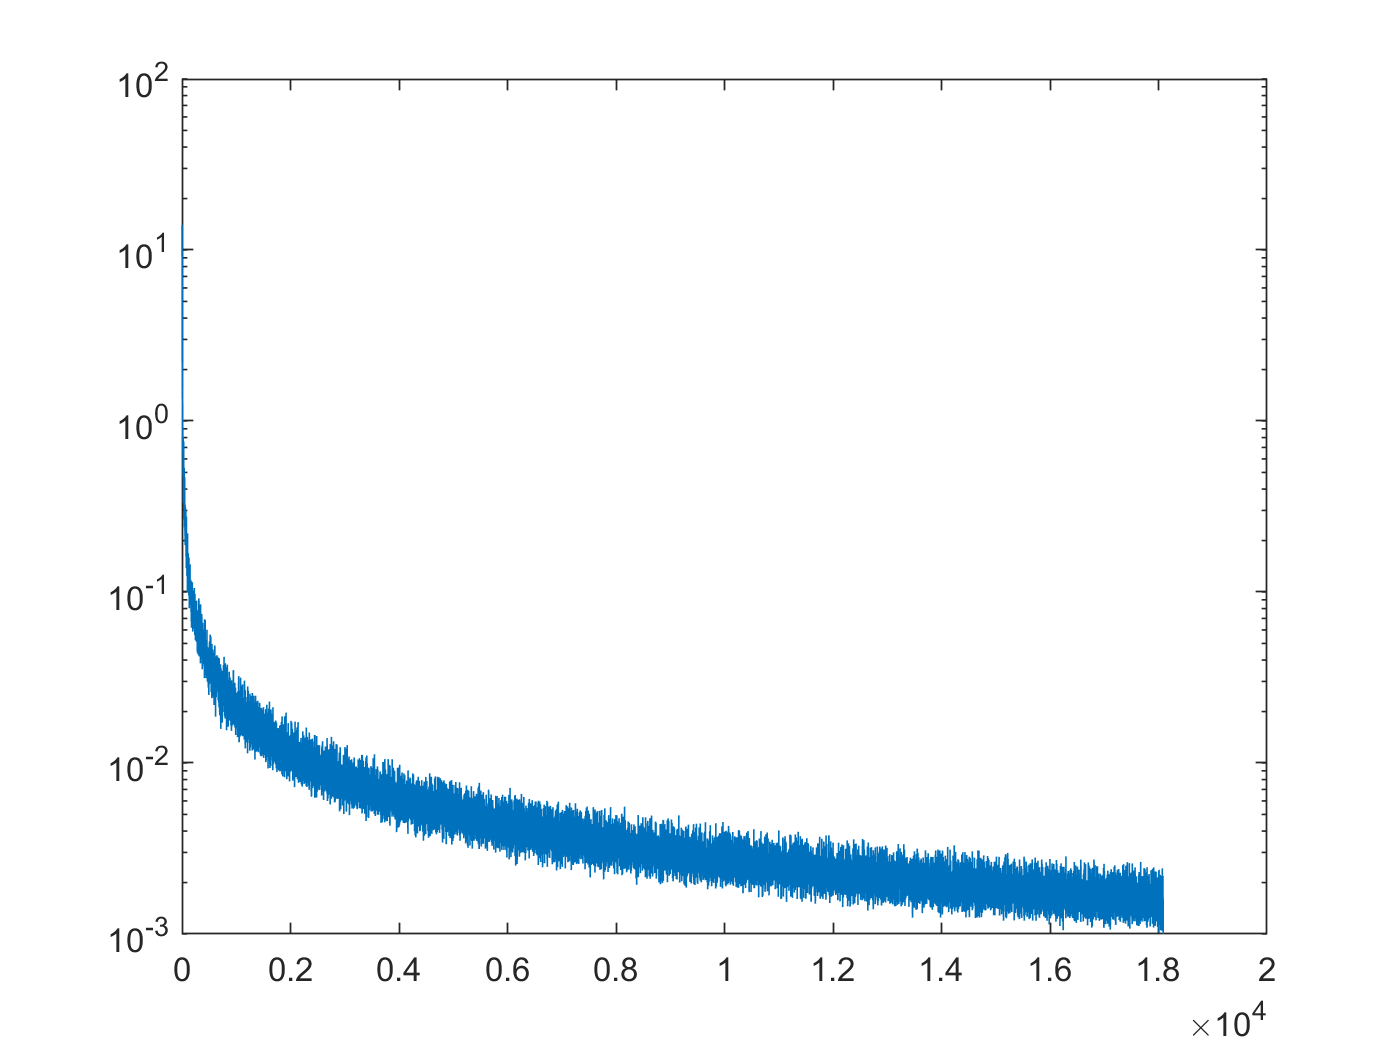
\includegraphics[width=0.8\textwidth]{gaps.png}
    \caption{Plot of the Frank-Wolfe gap versus the number of iterations.}
    \label{fig:my_label}
\end{figure}
\pagebreak
\subsection*{Question 14} 
We can see that the solution we compute is sparser than then one obtained by the Matlab solver. This is due to the fact that the Matlab solver doesn't enforce that the solution is contained in \(\Delta^n\).
\begin{figure}[h]
    \centering
    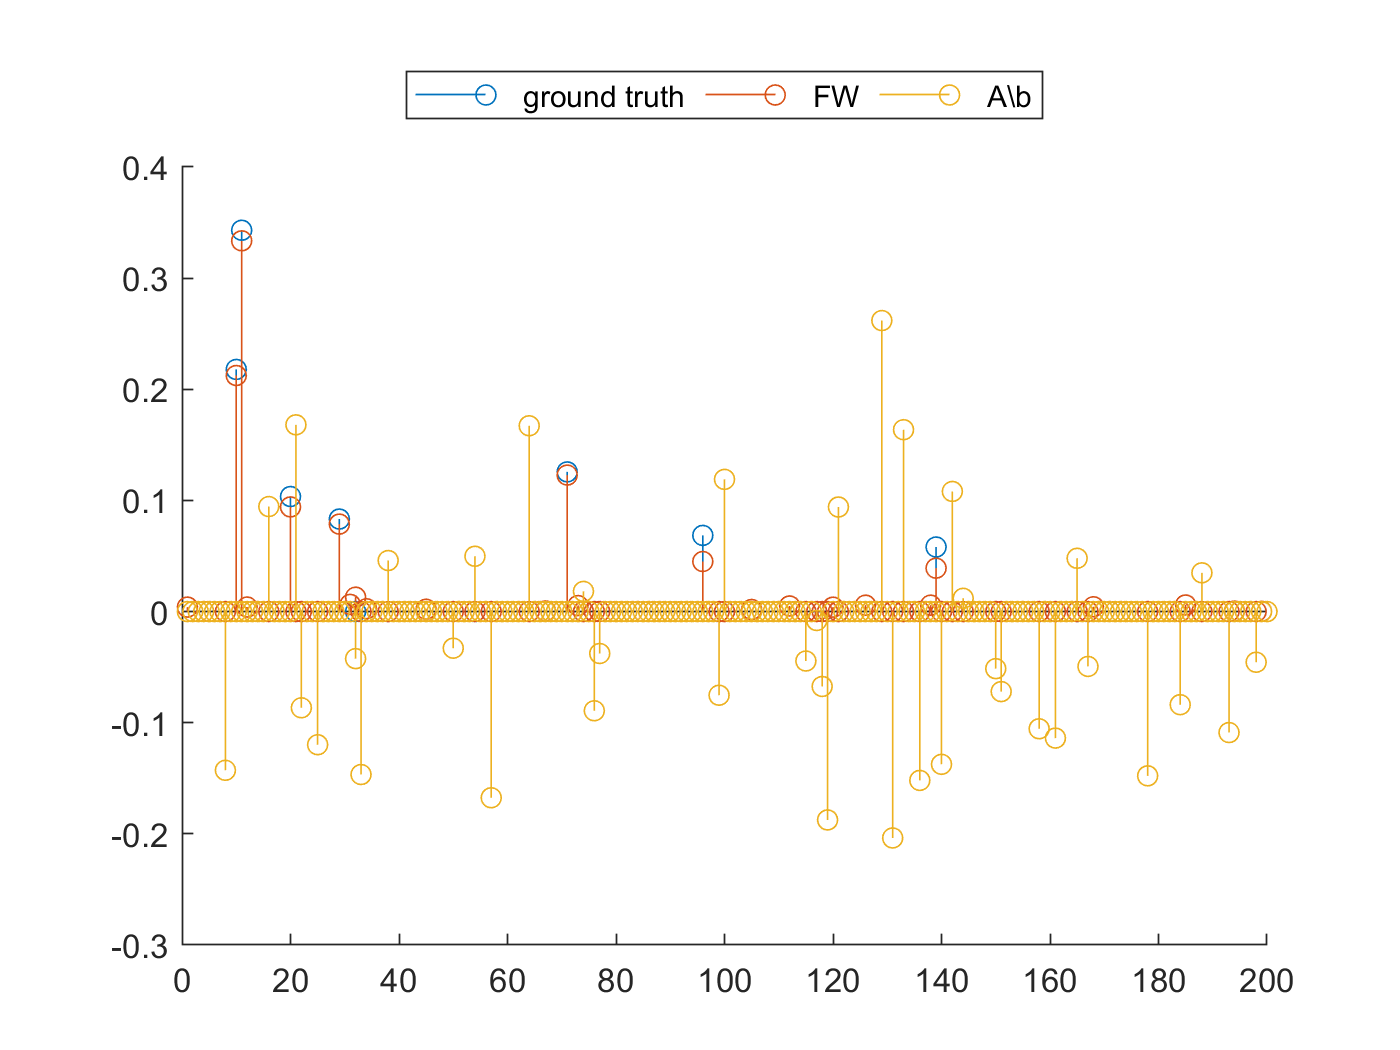
\includegraphics[width=0.5\textwidth]{compare.png}
    \caption{Comparison of the Frank-Wolfe algorithm, the true value and the vector obtained by the Matlab solver.}
    \label{fig:next}
\end{figure}

\pagebreak


\section*{Part 3 : KKT conditions and constraint qualifications}

\subsection*{Question 1}\hfil\par
Notice that:
\[f_i(x)\leq y;\ \forall \ i=1,\dots,N\iff\]
\[\max_{i=1,\dots,N}f_i(x)\leq y\iff \]
\[f(x)\leq y \implies \]
\[\min_xf(x)\leq\min_{(x,y)\in S}y\]

The other inequality is trivial as \((x,f(x))\in S\). So we can easily conclude that the 2 programs have the same optimal value.

\subsection*{Question 2}\hfil\par
Notice that the constraints for \(S\) are:

\[
    g_i(x,y)=f_i(x)-y\leq 0;\ \forall \ i=1,\dots,N
\]

It is easy to see that:
\[
    \nabla g_i(x,y)=\begin{pmatrix}
    \nabla f_i(x)\\
     -1
    \end{pmatrix}    
\]

The KKT conditions for \((x,y)\in S\) are: \((x,y)\) is a KKT point if there exists \(\lambda\in\mathbb{R}^N\), with \(\lambda\geq0\) such that:
\[
    -(0,\dots,0,1)=   \sum_{i=1}^{N}\lambda_i(\nabla f_i(x)^T,-1)    
\]
and
\[
    \lambda_i(f_i(x)-y)=0;\ \forall\ i=1,\dots,N  
\]
\subsection*{Question 3}\hfil\par
Let \(n=1\) and:
\[
    f_1(x)=x,\ f_2(x)=x^2,\ f_3(x)=x^3
\]

Then:
\[
  \nabla g_1(x,y)=\begin{pmatrix}
    1\\
     -1
    \end{pmatrix},\ \nabla g_2(x,y)=\begin{pmatrix}
    2x\\
     -1
    \end{pmatrix},\ \nabla g_3(x,y)=\begin{pmatrix}
    3x^2\\
     -1
    \end{pmatrix}
\]

For \((x,y)=(1,1)\in S\), it is clear that LICQ doesn't hold as \(\nabla g_1(1,1),\ \nabla g_2(1,1),\ \nabla g_3(1,1)\) are linearly dependent as a family of 3 vectors in \(\mathbb{R}^2\) (\(g_i(1,1)=0\) for all \(i\)).

\subsection*{Question 4}\hfil\par
Let \(I(x,y)=\{i\in\{1,\dots ,N\}\ |\ g_i(x,y)=0\}\). Then for MFCQ to hold, for all \((x,y)\in S\) we need to find a point \((\tilde x, \tilde y)\in S\) such that:
\[
  \langle \nabla g_i(x,  y), (\tilde x- x, \tilde y-y)\rangle<0;\ \forall\ i\in I(x)
\]
Substituting \(\nabla g_i\), we need to find \((\tilde x, \tilde y)\in S\) such that:
\[
    \left\langle \begin{pmatrix}
        \nabla f_i(x)\\
         -1
        \end{pmatrix}    , (\tilde x- x, \tilde y-y)\right\rangle<0;\ \forall\ i\in I(x)
\]
But notice that if we set \(\tilde x:=x\) and \(\tilde y:=y+1\) then:
\[
    \left\langle \begin{pmatrix}
        \nabla f_i(x)\\
         -1
        \end{pmatrix}    , (0, 1)\right\rangle=\langle-1,1\rangle=-1<0;\ \forall\ i\in I(x)
\]

So MFCQ holds for all \((x,y)\in S\).

(\textbf{Note}:\((x,y+1)\in S\) as \(y+1>y\geq f_i(x)\), for all \(i\))
\end{document}
























































